% !TeX program = pdfLaTeX
\documentclass[12pt]{article}
\usepackage{amsmath}
\usepackage{graphicx,psfrag,epsf}
\usepackage{enumerate}
\usepackage{natbib}
\usepackage{textcomp}
\usepackage[hyphens]{url} % not crucial - just used below for the URL
\usepackage{hyperref}
\providecommand{\tightlist}{%
  \setlength{\itemsep}{0pt}\setlength{\parskip}{0pt}}

%\pdfminorversion=4
% NOTE: To produce blinded version, replace "0" with "1" below.
\newcommand{\blind}{0}

% DON'T change margins - should be 1 inch all around.
\addtolength{\oddsidemargin}{-.5in}%
\addtolength{\evensidemargin}{-.5in}%
\addtolength{\textwidth}{1in}%
\addtolength{\textheight}{1.3in}%
\addtolength{\topmargin}{-.8in}%

%% load any required packages here
\setlength {\marginparwidth }{2cm}

\usepackage{mathtools,amssymb,booktabs,longtable,todonotes,amsthm} \def\mod{~\text{mod}~}



\usepackage{booktabs}
\usepackage{longtable}
\usepackage{array}
\usepackage{multirow}
\usepackage{wrapfig}
\usepackage{float}
\usepackage{colortbl}
\usepackage{pdflscape}
\usepackage{tabu}
\usepackage{threeparttable}
\usepackage{threeparttablex}
\usepackage[normalem]{ulem}
\usepackage{makecell}
\usepackage{xcolor}

\begin{document}


\def\spacingset#1{\renewcommand{\baselinestretch}%
{#1}\small\normalsize} \spacingset{1}


%%%%%%%%%%%%%%%%%%%%%%%%%%%%%%%%%%%%%%%%%%%%%%%%%%%%%%%%%%%%%%%%%%%%%%%%%%%%%%

\if0\blind
{
  \title{\bf Visualizing probability distributions across bivariate cyclic temporal granularities}

  \author{
        Sayani Gupta \thanks{Email: \href{mailto:Sayani.Gupta@monash.edu}{\nolinkurl{Sayani.Gupta@monash.edu}}} \\
    Department of Econometrics and Business Statistics, Monash University\\
     and \\     Rob J Hyndman \\
    Department of Econometrics and Business Statistics, Monash University\\
     and \\     Dianne Cook \\
    Department of Econometrics and Business Statistics, Monash University\\
     and \\     Antony Unwin \\
    University of Augsburg\\
      }
  \maketitle
} \fi

\if1\blind
{
  \bigskip
  \bigskip
  \bigskip
  \begin{center}
    {\LARGE\bf Visualizing probability distributions across bivariate cyclic temporal granularities}
  \end{center}
  \medskip
} \fi

\bigskip
\begin{abstract}
Deconstructing a time index into time granularities can assist in exploration and automated analysis of large temporal data sets. This paper describes several classes of time deconstructions using linear and cyclic time granularities. Linear time granularities respect the linear progression of time such as hours, days, weeks and months with respect to a baseline. Cyclic time granularities can be circular such as hour of the day, quasi-circular such as day of the month, and aperiodic such as public holidays. The hierarchical structure of granularities creates a nested ordering. Hour of the day and second of the minute are single-order-up. Hour of the week is multiple-order-up, because it passes over day of the week. Methods are provided for creating all possible granularities for a time index. A recommendation algorithm provides an indication whether a pair of granularities can be meaningfully examined together, called a harmony or when they cannot, called a clash.

The time granularities can be used to create visualizations of the data to explore for periodicities, associations and anomalies. The granularities can be considered to be categorical variables (ordered or unordered) which induces a grouping of the observations. Assuming a numeric response variable, the resulting graphics are then displays of distributions compared across combinations of categorical variables. A recommendation of appropriate distribution display is provided.

The methods are implemented in the open source R package \texttt{gravitas}. The functions for creating granularities and exploring the associated time series are consistent with a tidy workflow (\citet{Grolemund2018-po}), and the probability distributions can be examined using the range of graphics available in \texttt{ggplot2} \citep{Wickham2009pk}.
\end{abstract}

\noindent%
{\it Keywords:} data visualization, statistical distributions, time granularities, calendar algebra, periodicties, grammar of graphics, R
\vfill

\newpage
\spacingset{1.45} % DON'T change the spacing!

\hypertarget{introduction}{%
\section{Introduction}\label{introduction}}

Temporal data are available at various resolutions depending on the context. Social and economic data like GDP is often collected and reported at coarse temporal scales such as monthly, quarterly or annually. With recent advancement in technology, more and more data are recorded at much finer temporal scales. Energy consumption may be collected every half an hour, energy supply may be collected every minute, and web search data might be recorded every second. As the frequency of data increases, the number of questions about the periodicity of the observed variable also increases. For example, data collected at an hourly scale can be analyzed using coarser temporal scales such as days, months or quarters. This approach requires deconstructing time in various possible ways called time granularities \citep{aigner2011visualization}.

It is important to be able to navigate through all of these time granularities to have multiple perspectives on the periodicity of the observed data. This idea aligns with the notion of EDA \citep{Tukey1977-jx} which emphasizes the use of multiple perspectives on data to help formulate hypotheses before proceeding to hypothesis testing. Visualizing probability distributions conditional on one or more granularities is an indispensable tool for exploration. Analysts are expected to comprehensively explore the many ways to view and consider temporal data. However, the plethora of choices and the lack of a systematic approach to do so quickly becomes overwhelming.

Calendar-based graphics \citep{wang2020calendar} are useful in visualizing patterns in the weekly and monthly structure, and are helpful when checking for the effects of weekends or special days. Any temporal data at sub-daily resolution can also be displayed using this type of faceting \citep{Wickham2009pk} with days of the week, month of the year, or another sub-daily deconstruction of time. But calendar effects are not restricted to conventional day-of-week or month-of-year deconstructions. There can be many different time deconstructions, based on the calendar or on categorizations of time granularities.

Linear time granularities respect the linear progression of time and are non-repeating such as hours, days, weeks and months. One of the first attempts to characterize these granularities is due to \citet{Bettini1998-ed}. However, the definitions and rules defined are inadequate for describing cyclic or repeating granularities. Hence, there is a need to define some new cyclic time granularities, that can be useful in visualizations. Cyclic time granularities can be circular, quasi-circular or aperiodic. Examples of circular granularities are hour of the day and day of the week; an example of a quasi-circular granularity is day of the month; examples of aperiodic granularities are public holidays and school holidays.

Time deconstructions can also be based on the hierarchical structure of time. For example, hours are nested within days, days within weeks, weeks within months, and so on. Hence, it is possible to construct single-order-up granularities such as second of the minute, or multiple-order-up granularities such as second of the hour. The lubridate package \citep{Grolemund2011-vm} provides tools to access and manipulate common date-time objects. However, most of its accessor functions are limited to single-order-up granularities.

The motivation for this work stems from the desire to provide methods to better understand large quantities of measurements on energy usage reported by smart meters in households across Australia, and indeed many parts of the world. Smart meters currently provide half-hourly use in kWh for each household, from the time that they were installed, some as early as 2012. Households are distributed geographically and have different demographic properties such as the existence of solar panels, central heating or air conditioning. The behavioral patterns in households vary substantially, for example, some families use a dryer for their clothes while others hang them on a line, and some households might consist of night owls, while others are morning larks. It is common to see aggregates \citep[see][]{Goodwin_2012} of usage across households, such as half-hourly total usage by state, because energy companies need to plan for maximum loads on the network. But studying overall energy use hides the distribution of usage at finer scales, and makes it more difficult to find solutions to improve energy efficiency. We propose that the analysis of smart meter data will benefit from systematically exploring energy consumption by visualizing the probability distributions across different deconstructions of time to find regular patterns/anomalies. Although, the motivation came through the smart meter example, this is a problem that is relevant to any temporal data observed more than once per year.

This work provides tools for systematically exploring bivariate granularities within the tidy workflow. In particular, we

\begin{itemize}
\tightlist
\item
  provide a formal characterization of cyclic granularities;
\item
  facilitate manipulation of single- and multiple-order-up time granularities through cyclic calendar algebra;
\item
  develop an approach to check the feasibility of creating plots or drawing inferences for any two cyclic granularities;
\item
  recommend prospective probability distributions for exploring distributions of a univariate dependent variable across pair of granularities.
\end{itemize}

The remainder of the paper is organized as follows: Section \ref{sec:linear-time} provides some background material on linear granularities and calendar algebra for computing different linear granularities. Section \ref{sec:cyclic-gran} formally characterizes different cyclic time granularities by extending the framework of linear time granularities. Section \ref{sec:cyclic-calendar} introduces cyclic calendar algebra for computing cyclic time granularities. Section \ref{sec:data-structure} discusses the data structure for exploring the conditional distributions of the associated time series across pairs of cyclic time granularities. Section \ref{sec:visualization} discusses the role of different factors in constructing an informative and trustworthy visualization. Section \ref{sec:application} examines how systematic exploration can be carried out for a temporal and non-temporal application. Section \ref{sec:discussion} summarizes this paper and discusses possible future direction.

\hypertarget{sec:linear-time}{%
\section{Linear time granularities}\label{sec:linear-time}}

Discrete abstraction of time such as weeks, months or holidays can be thought of as ``time granularities''. Time granularities are \textbf{linear} if they respect the linear progression of time. There have been several attempts to provide a framework for formally characterizing time granularities, including \citet{Bettini1998-ed} which forms the basis of the work described here.

\hypertarget{definitions}{%
\subsection{Definitions}\label{definitions}}

\newtheorem{definition}{Definition}

\begin{definition}\label{def:definition}
A {\bf time domain} is a pair $(T; \le)$ where $T$ is a non-empty set of time instants and $\le$ is a total order on $T$.
\end{definition}

The time domain is assumed to be \emph{discrete}, and there is unique predecessor and successor for every element in the time domain except for the first and last.

\begin{definition}\label{def:index set}
There is a unique {\bf index set}, $Z=\{z: z \in \mathbb{Z}_{\geq 0}\}$, which map the time instants to a set of non-negative integers. Often, this is thought of as $t=0, \dots, T$.
\end{definition}

\begin{definition}\label{def:linear}
A {\bf linear granularity} is a mapping $G$ from the integers (the index set, $Z$) to subsets of the time domain such that:
  (1) if $i < j$ and $G(i)$ and $G(j)$ are non-empty, then each element of $G(i)$ is less
than all elements of $G(j)$; and
  (2) if $i < k < j$ and $G(i)$ and $G(j)$ are non-empty, then $G(k)$ is non-empty.
Each non-empty subset $G(i)$ is called a {\bf granule}.
\end{definition}

\noindent This implies that the granules in a linear granularity are non-overlapping, continuous and ordering is maintained. The indexing for each granule can also be associated with textual representation, called the label. A discrete time model often uses a fixed smallest linear granularity named by \citet{Bettini1998-ed} \textbf{bottom granularity}. \autoref{fig:linear-time} illustrates the linear time granularities. Here, ``hour'' is the bottom granularity and ``day'', ``week'', ``month'' and ``year'' are linear granularities which maps from index set to subsets of the hourly time domain. If we have ``hour'' running from \(\{0, 1, \dots,t\}\), we will have ``day'' running from \(\{0, 1, \dots, \lfloor t/24\rfloor\}\). These linear granularities are ordered with ordering guided by the index set which is a set of integers. Hence, they are uni-directional and non-repeating.

\begin{figure}

{\centering 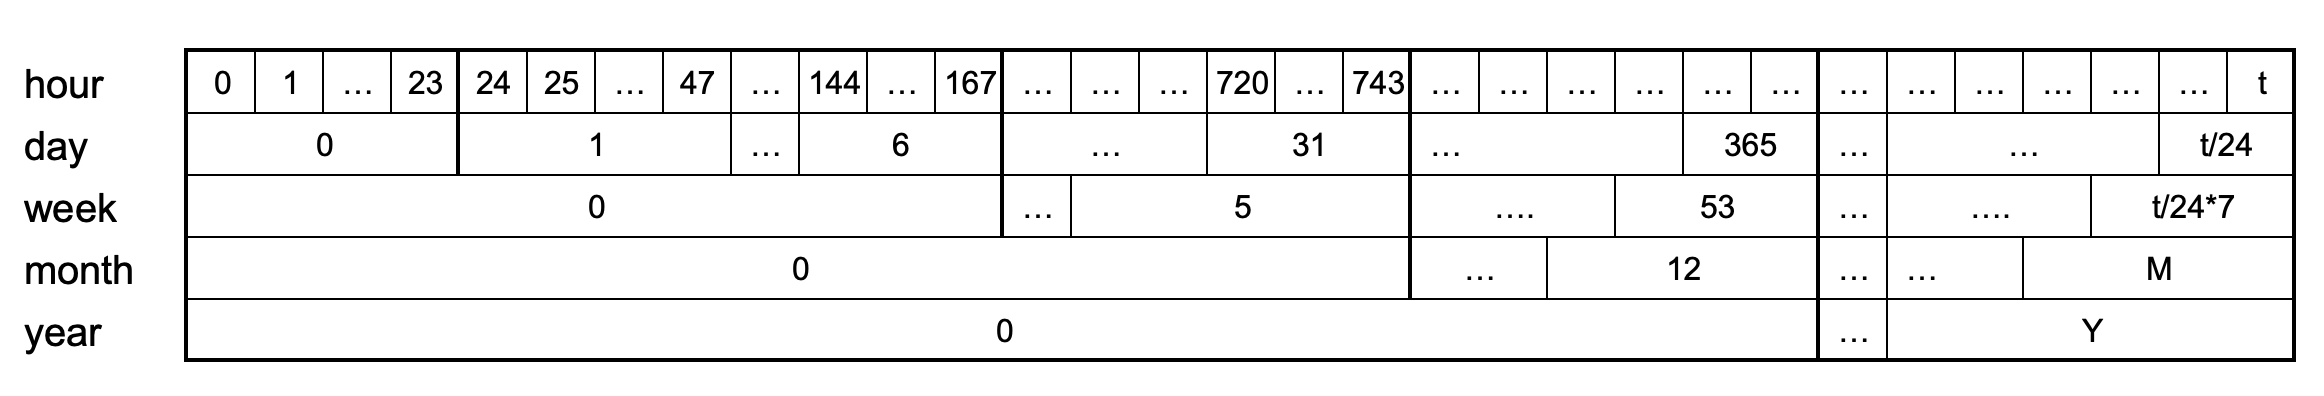
\includegraphics[width=1\linewidth]{Figs/linear-ex} 

}

\caption{Illustration of time domain, linear granularities and index set. Hour, day, week, month and year are linear granularities and can also be considered to be time domains. These are ordered with ordering guided by integers and hence is unidirectional and non-repeating. Hours could also be considered the index set, and a bottom granularity.}\label{fig:linear-time}
\end{figure}



\hypertarget{relativities}{%
\subsection{Relativities}\label{relativities}}

Properties of pairs of granularities fall into various categories.

\begin{definition}\label{def:finerthan}
A linear granularity $G$ is {\bf finer than} a linear granularity $H$, denoted $G \preceq H$, if for each index $i$, there exists an index $j$ such that
$G(i) \subset H(j).$
\end{definition}

\begin{definition}\label{def:groupsinto}
A linear granularity $G$ {\bf groups into} a linear granularity $H$, denoted
$G \trianglelefteq H$, if for each index $j$ there exists a (possibly infinite) subset $S$ of the integers such that $H(j) = \bigcup_{i \in S}G(i).$
\end{definition}

\newtheorem*{example}{Example}

\begin{example}
{\rm Both $day \trianglelefteq week$ and $day \preceq week$ holds, since every granule of $week$ is the union of some set of granules of day and each day is a subset of a $week$. Consider another example where $day \trianglelefteq month$. This relationship however is incomplete without its association to periodicity. Each month is a grouping of the same number of days over years, hence the period of the grouping $(day, month)$ is one year, if leap years are ignored. This grouping period becomes 4 and 400 years with the inclusion of leap years and leap seconds respectively.}
\end{example}

\begin{definition}\label{def:periodical}
A granularity $G$ is {\bf periodical} with respect to a granularity $H$ if:
(1) $G \trianglelefteq H$; and
(2) there exist $R$, $P \in \mathbb{Z}_+$, where $R$ is less than the number of granules of $H$, such that for all $i \in \mathbb{Z}$, if $H(i) = \bigcup_{j \in S}G(j)$ and $H (i + R) \neq \phi$ then $H (i + R) = \bigcup_{j \in S} G(j + P)$.
\end{definition}

If \({S_0,\dots,S_{R-1}}\) are the sets of indexes of \(G\) describing
\(H(0), \dots, H(R - 1)\), respectively, then the description of an arbitrary granule \(H(j)\) is given by \(\bigcup_{i \in S_j ~\text{mod}~R}G(P*\lfloor j/R \rfloor + i)\). Also, granularities can be periodical with respect to other granularities, except for a finite number of spans of time where they behave in an anomalous way, called \textbf{quasi-periodic} relationships by \citet{Bettini2000-vy}.

\begin{example}
{\rm In a Gregorian calendar without leap years we could say $day$ groups periodically into month with the period $P = 365$ and the number of granules of $month$ in each period given by $R=12$. In a Gregorian calendar with leap years, $day$ groups quasi-periodically into $month$ with the exceptions of the time domain corresponding to $29^{\text{th}}$ February of any year.}
\end{example}

\begin{definition}\label{def:order}
The {\bf order} of a linear granularity is the level of coarseness associated with a linear granularity. A linear granularity G will have lower order than H if each granule of G is composed of lower number of granules of bottom granularity than each granule of H.
\end{definition}

\begin{example}
{\rm For two linear granularities $G$ and $H$, if $G$ {\em groups into} or {\em finer than} $H$ then $G$ is of lower order than $H$. Moreover, if we consider bottom granularity as day, linear granularity week will have lower order than month since each week consist of less number of days than each month. Here neither  week {\em groups into} month or  week {\em finer than} month, but their relative order could be determined.}
\end{example}

\hypertarget{computation}{%
\subsection{Computation}\label{computation}}

Granules in bottom granularity or any finer granularity may be aggregated in some manner to form larger granules belonging to a coarser granularity. A system of multiple granularities in lattice structures is referred to as a \textbf{calendar} by \citet{Dyreson_2000}. Linear time granularities are computed through an algebraic representation for time granularities, which is referred to as calendar algebra \citep{Ning_2002}. It is assumed that there exists a \emph{bottom granularity} and calendar algebra operations are designed to generate new granularities recursively from the bottom one. Some relevant calendar algebra operations are discussed below; these will be used in Section \ref{sec:cyclic-gran} for illustrations in circular and quasi-circular granularities.

\begin{definition}\label{def:grouping_operation}
Let $G_1$ be a full-integer labelled granularity, and $m$ a positive integer. {\bf The grouping operation} Group$_m(G)$ generates a new granularity $G_2$, by partitioning the granules of $G_1$ into $m$-granule groups and making each group a granule of the resulting granularity. More precisely, $G_2 = \text{Group}_m(G_1)$ is the full-integer labelled granularity such that for each integer $i$,
$$G_2(i) = \bigcup\limits_{j = (i-1)m+1}^{im} G_1(j).$$
The grouping operation Group$_m(G)$, provides a new granularity whose granules are the integer part of the quotient when the integer set spanned by linear granularity $G$ is divided by $m$, such that, $G_2(i) = \lfloor G_1(j)/m \rfloor$.
\end{definition}

\begin{example} 
{\rm Due to even length of $day$ and $week$, we can derive them from $hour$ using the grouping operation as follows: day = G$_{24}(\text{hour})$, week = G$_{24*7}(\text{hour})$.}
\end{example}

\noindent For more variations of calendar algebra operations, see \citet{Ning_2002}.

\hypertarget{sec:cyclic-gran}{%
\section{Cyclic time granularities}\label{sec:cyclic-gran}}

Cyclic granularities represent cyclical repetitions in time. They can be thought of as additional categorizations of time that are not linear. Cyclic granularities can be constructed by operating on two linear granularities. Cycles can be either \emph{regular}, called \textbf{circular}, or \emph{irregular}, \textbf{quasi-circular} when these two linear granularities relate periodically.

\hypertarget{sec:circular-gran-def}{%
\subsection{Circular}\label{sec:circular-gran-def}}

\begin{definition}\label{def:circular}
A {\bf circular granularity} $C_{B, G}$ relates a linear granularity $G$ to the bottom granularity B, if
\begin{equation} \label{eq:circular-gran}
\begin{split}
C_{B, G}(z) & = z~\text{mod}~P(B, G) \quad \forall z \in \mathbb{Z}_{\geq 0} \\
\end{split}
\end{equation}
where
z denotes the index set,
B denotes a full-integer labelled bottom granularity which groups periodically into linear granularity $G$ with regular mapping, and $P \equiv P(B, G)$ is the number of granules of $B$ in each granule of $G$, also called the period of the grouping $(B, G)$.
\end{definition}

\begin{example}
{\rm \autoref{fig:circular-dow} illustrates the linear and the corresponding cyclical granularities. Cyclical granularities can be considered to be cutting the linear granularity into pieces, and stacking them to match the cycles (as shown in b). $B, G, H$ (day, week, fortnight, respectively) are linear granularities. The circular granularity $C_{B , G}$ (day-of-week)is constructed from $B$ and  $G$. The circular granularity $C_{B, H}$ (day-of-fortnight) is constructed from $B$ and $H$. These overlapping cyclical granularities share elements from the linear granularity. Each of $C_{B , G}$ and $C_{B , H}$ consist of repeated patterns  $\{0, 1, 2, \dots, 6\}$ and $\{0, 1, 2, \dots, 13\}$ with $P=7$ and $P=14$ respectively. Each circular granularity can use descriptive label mappings. Suppose ${L}$ is a label mapping that defines an unique label for each index $l \in \{ 0,1,\dots, (P-1)\}$, then the label mapping $L$ for $C_{B, G}$ can be defined as
$$
  L: \{0,1,2, \dots, 6\} \longmapsto\ \{\text{Sun}, \text{Mon}, \dots, \text{Sat}\}
$$
or
$$
  L: \{0,1,2, \dots, 6\} \longmapsto\ \{\text{Sunday}, \text{Monday}, \dots, \text{Saturday}\}
$$
for example.}
\end{example}

\begin{figure}

{\centering 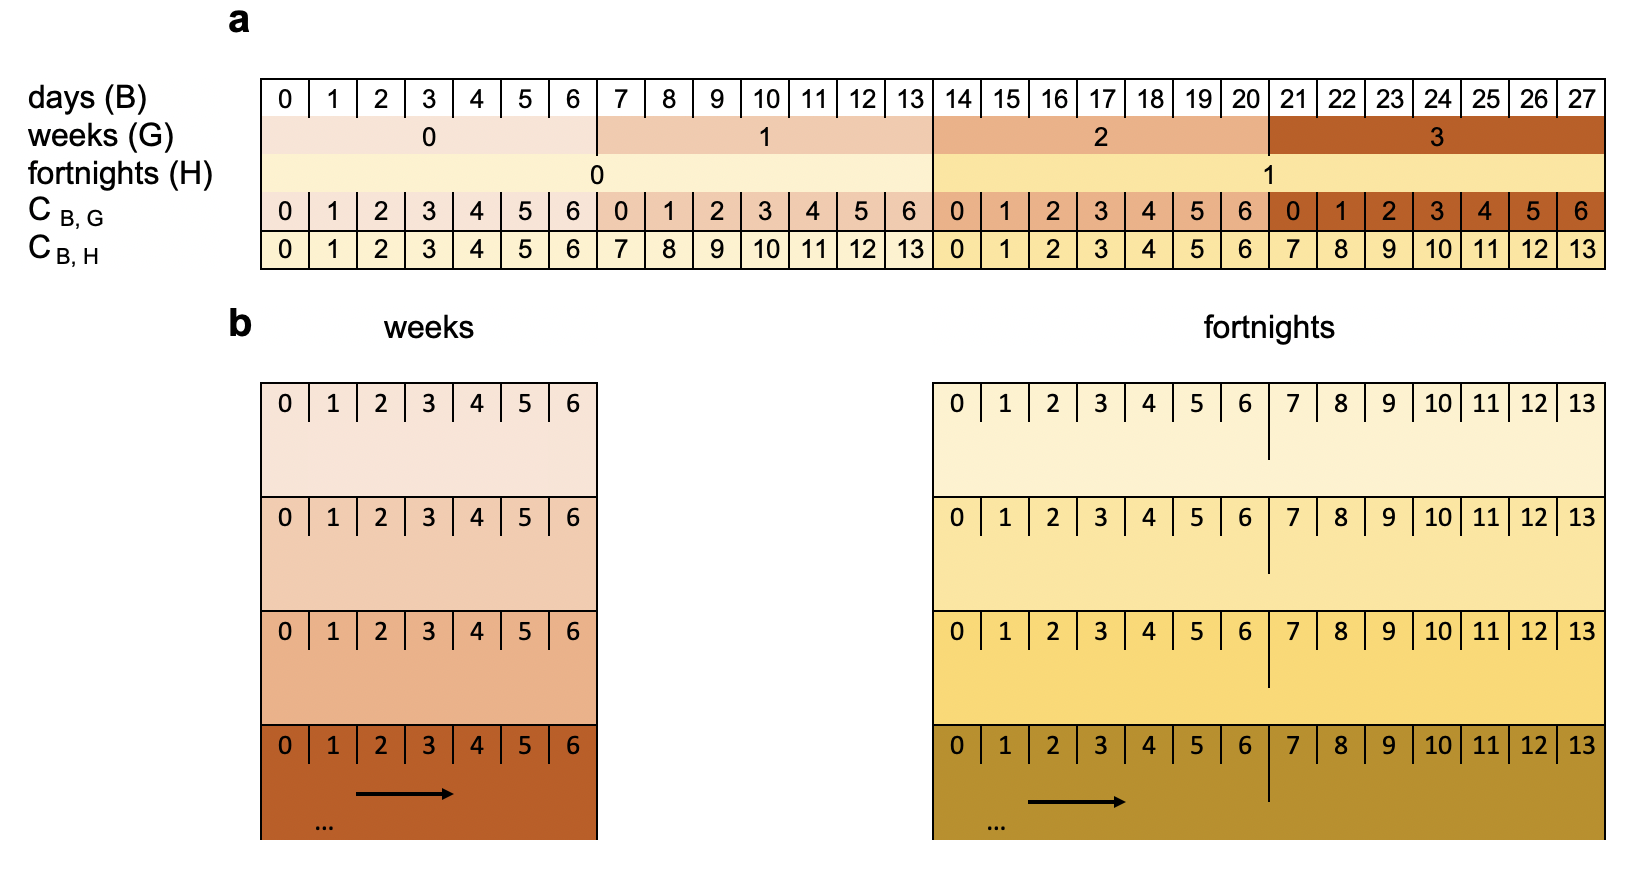
\includegraphics[width=1\linewidth]{Figs/circular-ex} 

}

\caption{Illustration of circular relative to linear granularities (a). Circular granularities can be considered to be cutting the linear granularity into pieces and stacking them (b). The circular granularity creates repeated integer sequences.}\label{fig:circular-dow}
\end{figure}



In general, any circular granularity relating two linear granularity can be expressed as \(C_{(G, H)}(z) = \lfloor z/P(B,G) \rfloor~\text{mod}~P(G,H)\), where linear granularity \(H\) is periodic with respect to linear granularity \(G\) with regular mapping and \(P(G,H)\) is the period of the grouping \((G, H)\) . Table \ref{tab:definitions} shows representation of circular granularities \(C_i\) relating two linear granularities with period \(P_i\) and minutes as the bottom granularity.

\begin{table}[ht]
\begin{center}
\begin{tabular}{lll}
\hline
circular granularity & expression & period \\
\hline
minute-of-hour                               &
  $C_1 = z ~\text{mod}~60$                     &
  $P_1 = \phantom{99}60$ \\
minute-of-day                                &
  $C_j = z ~\text{mod}~60*24$                  &
  $P_2= 1440$\\
hour-of-day                                  &
  $C_3 = \lfloor z/60\rfloor~\text{mod}~24$    &
  $P_3 = \phantom{99}24$ \\
hour-of-week                                 &
  $C_4 = \lfloor z/60\rfloor~\text{mod}~24*7$  &
  $P_4= \phantom{9}168$\\
day-of-week                                  &
  $C_5 = \lfloor z/24*60\rfloor ~\text{mod}~7$ &
  $P_5= \phantom{999}7$\\
\bottomrule
\end{tabular}
\end{center}
\caption{Examples of circular granularities with bottom granularity minutes. Circular granularity $C_i$ relates two linear granularities one of which groups periodically into the other with regular mapping and period $P_i$. Circular granularities can be expressed using modular arithmetic due to their regular mapping. }
\label{tab:definitions}
\end{table}

\hypertarget{sec:quasi-circular-gran-def}{%
\subsection{Quasi-circular}\label{sec:quasi-circular-gran-def}}

A \textbf{quasi-circular} granularity can not be defined using modular arithmetic since they are formed using two linear granularities with irregular mapping. However, they are still formed with linear granularities, one of which ``groups periodically into'' the other. \autoref{tab:quasi} shows some example of quasi-circular granularities (\(Q_i\)) with (\(P_i\)) denoting the plausible choices of period of the grouping of two linear granularities.

\begin{table}[ht]
\begin{center}
\begin{tabular}{lr@{~}lr@{~}r}
\hline
quasi-circular granularity && potential period lengths\\
\hline
$Q_1 =$ day-of-month && $P_1 = 31, 30, 29, 28$\\
$Q_2 =$ hour-of-month && $P_2 = 24*31, 24*30, 24*29, 24*28$\\
$Q_3 =$ day-of-year && $P_3 = 366, 365$\\
$Q_4 =$ week-of-month && $P_4 = 5, 4$\\
\bottomrule
\end{tabular}
\end{center}
\caption{Examples of quasi-circular granularities $Q_i$ with potential period lengths $P_i$. These quasi-circular granularities relate two linear granularities one of which groups periodically into the other with irregular mapping leading to many potential period lengths and hence can not be expressed through modular arithmetic. }
\label{tab:quasi}
\end{table}

\begin{definition}\label{def:quasicircular}
A {\bf quasi-circular granularity} $Q_{B, G'}$ relates linear granularities $G'$ and bottom granularity $B$, if
\begin{equation}\label{eq:quasi}
\begin{split}
Q_{B, G'}(z) =
z - \sum_{w=0}^{k-1}\vert T_{w ~\text{mod}~R'} \vert, & \quad \text{for}\quad z \in T_{k}
\end{split}
\end{equation}
where,
$z \in \mathbb{Z}_{\geq 0}$ denotes the index set,
$B$ denotes a full-integer labelled bottom granularity which groups periodically into linear granularity $G'$ with irregular mapping, $P'$ and $R'$ are the period of the grouping $(B, G')$ and the number of granules of $G'$ in $P'$, $T_w$ are the sets of indices of $B$ describing $G'(w)$ such that  $G'(w) = \bigcup_{z \in T_w}B(z)$ and $\vert T_w \vert$ is the cardinality of set $T_w$.
\end{definition}

\begin{example}
{\rm Consider $G'$ such that every two consecutive granules of $G'$ are made up of $7$ and $5$ granules of $B$ respectively within each period of the grouping ($B$, $G'$). Then $Q_{B, G'}$ is a repetitive categorization of time, similar to circular granularities, except that the number of granules of $B$ is not necessarily the same across different granules of $G'$. Here, $T_0 = \{0, 1, 2, 3, 4, 5, 6\}$ and $T_1 = \{7, 8, 9, 10, 11\}$. Hence using Definition \autoref{def:quasicircular} we will have:

\begin{align*}
\begin{split}
Q_{B,H'}(10) & = 10 - \sum_{w=0}^{1-1}\vert T_{w ~\text{mod}~2}\vert ,\quad since \quad 10 \in T_{1}  \\
  & = 3 \\
\end{split}
\end{align*}
}
\end{example}

If linear granularity \(G'\) is periodical with respect to \(B\) with irregular mapping, then there exist \(R'\), \(P' \in \mathbb{Z}_+\) such that if \(G'(w) = \bigcup_{z \in T_w}B(z)\) then \[G'(w) = \bigcup_{z \in T_w ~\text{mod}~R'}B(P'*\lfloor w/R' \rfloor + z)\] (from Definition \ref{def:periodical}) . Here \(w ~\text{mod}~R'\) represents the index that must be shifted to obtain \(G'(w)\). The idea here is if we know the composition of each of the granules of \(G'\) in terms of granules of \(B\) for one period, we can find the composition of any granule of \(G'\) beyond a period since the ``pattern'' repeats itself along the time domain due to the periodic property. The periodic property also ensures that \(\vert T_w \vert = \vert T_{w~\text{mod}~R'} \vert\) since every \(w^{\text{th}}\) and \((w+R')^{\text{th}}\) granule of \(G'\) will have the same number of granules of \(B\). The term \(\sum_{w=0}^{k-1}\vert T_{w}\vert\) in Definition \autoref{def:quasicircular} denotes the number of granules of \(B\) till the \((k-1)^{\text{th}}\) granule of \(G'\). Since \(\vert T_w \vert = \vert T_{w~\text{mod}~R'} \vert\), the number of granules of \(B\) till the \((k-1)^{\text{th}}\) granule of \(G'\) becomes \(\sum_{w=0}^{k-1}\vert T_{w ~\text{mod}~R'}\vert\) in Definition \autoref{def:quasicircular}.

\hypertarget{sec:aperiodic-gran-def}{%
\subsection{Aperiodic}\label{sec:aperiodic-gran-def}}

Aperiodic time granularities are the ones which can not be specified as a periodic repetition of a pattern of granules. Most public holidays repeat every year, but there is no reasonably small period within which their behavior remains constant. A classic example can be that of Easter, whose dates repeat only after 5,700,000 years. In Australia, if a standard public holiday falls on a weekend, a substitute public holiday will sometimes be observed on the first non-weekend day (usually Monday) after the weekend. Examples of aperiodic granularity may also include school holidays or a scheduled event. All of these are recurring events, but with non-periodic patterns. As such, plausible \(P_i\) from \autoref{tab:quasi} could be possibly infinite for aperiodic granularities.

\noindent Aperiodic cyclic granularities are defined using aperiodic linear granularities. Consider n aperiodic linear granularities \(M_i\) \(\forall \{i\in{1, 2, \dots, n\}}\) such that Definition \ref{def:periodical} does not hold true with respect to \(B\). However, \(B \trianglelefteq M_i\) \(\forall \{i\in{1, 2, \dots, n\}}\). Then according to Definition \ref{def:groupsinto}, for each index \(j\) there exists a (possibly infinite) subset \(T_{\{i_j\}}\) of the integers such that \(M_{i}(j) = \bigcup_{z \in T_{i_j}}B(z)\). Suppose \(M = \bigcup_{i=1}^{n}M_{i}\) is formed by collecting the granules of \(\{M_1, M_2, \dots, M_n\}\). Here, index \({\{i_j\}}\) stands for the \(j^{\text{th}}\) granule of the \(i^{\text{th}}\) linear aperiodic granularity.

\begin{figure}

{\centering 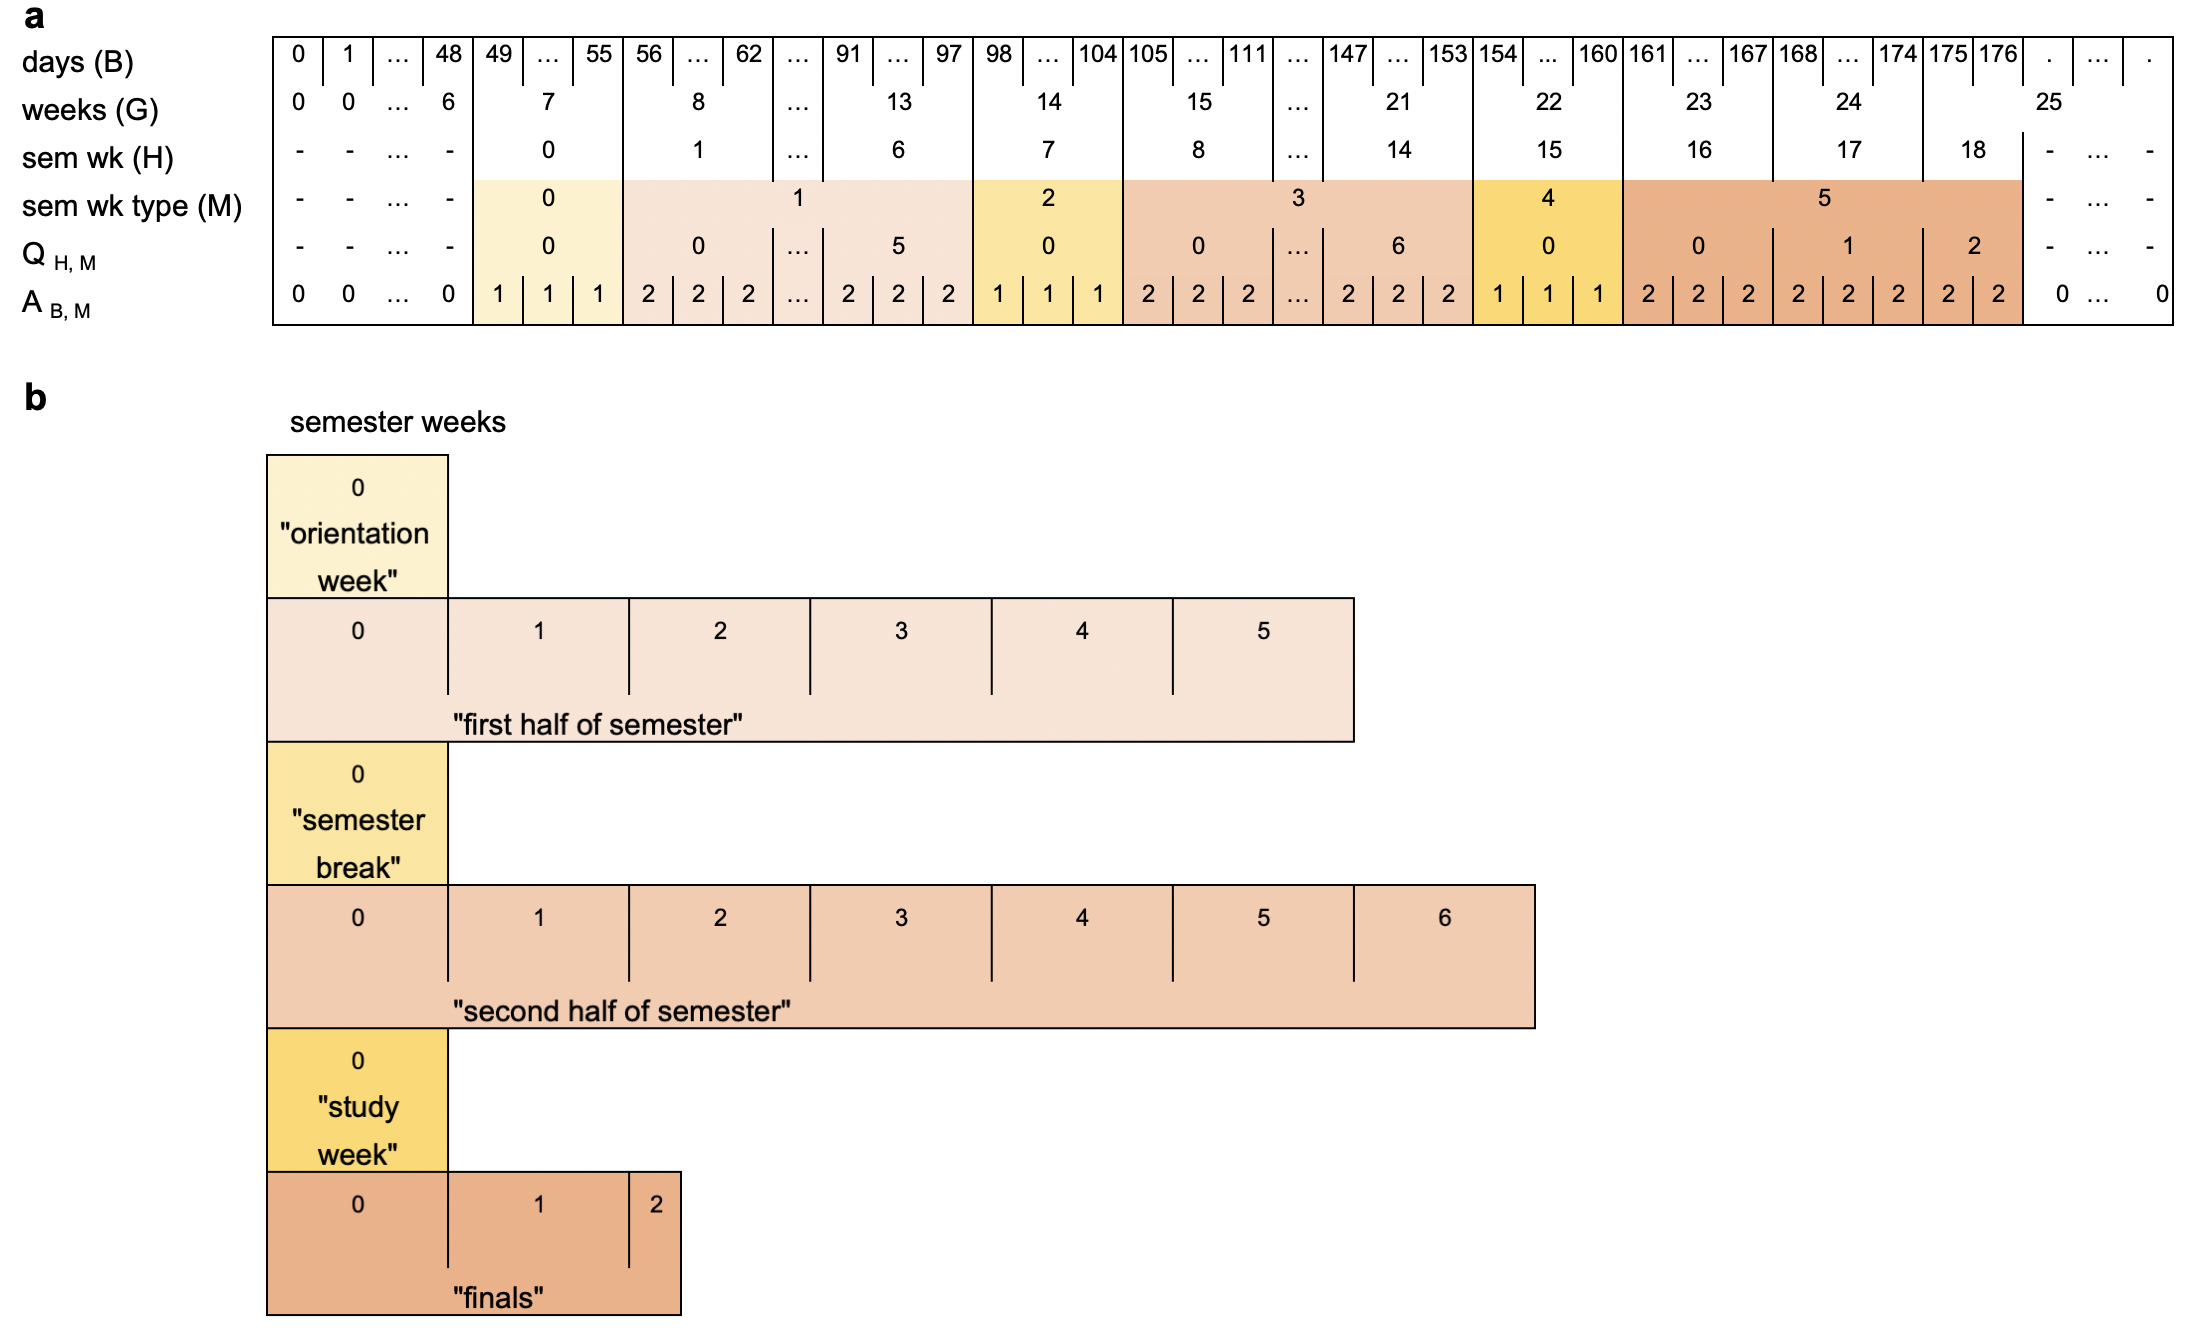
\includegraphics[width=1\linewidth]{Figs/aperiodic-ex3} 

}

\caption{Quasi-circular and aperiodic cyclic granularities illustrated through linear (a) and stack (b) display of time. The linear display shows linear granularities days, weeks, semester weeks, semester week type distributed linearly from past to future. Here a semester lasts for 18.3 weeks, each starting with one week of orientation followed by an in-session period of 6 weeks, a semester-break of 1 week and again an in-session period of 7 weeks and 1 week study break before final exams which continue for 1.3 weeks. This pattern remains same for all semester and hence \(Q_{H, M}\) with \(P\) = 18.3 weeks will be a quasi-circular granularity with repeating patterns. \(A_{B, M}\) will be an aperiodic cyclic granularity since the placement of the semester within an year varies across years.}\label{fig:aperiodic-example}
\end{figure}



\begin{definition}\label{def:aperiodic}
An {\bf aperiodic cyclic granularity} $A_{B, M}$ relates a linear granularity $M$ to the bottom granularity $B$, if
\begin{equation}\label{eq:aperiodic}
\begin{split}
A_{B, M}(z) & =
\begin{cases}
i, & \text{for}\quad z \in T_{i_j} \\
0  & \text{otherwise}
\end{cases}
\end{split}
\end{equation}
where,
$z \in \mathbb{Z}_{\geq 0}$ denotes the index set,
$B$ denotes a full-integer labelled bottom granularity which groups into linear granularity $M$ but not periodically, $T_{i_j}$ are the sets of indices of $B$ describing aperiodic linear granularities $M_{i}$ such that $M_{i}(j) = \bigcup_{z \in T_{i_j}}B(z)$, and $M = \bigcup_{i=1}^{n}M_{i}$.
\end{definition}

\begin{example}
{\rm Consider a school semester which always lasts for 18 weeks and 2 days, starting with one week of orientation followed by an in-session period of 6 weeks, a semester-break of 1 week and again an in-session period of 7 weeks and 1 week study break before final exams which continue for 16 days. Let the linear granularities $M_1$ and $M_2$ denote in-session semester period and semester break periods respectively. Both $M_1$, $M_2$ and $M = M_{1}\bigcup M_{2}$ denoting the semester week type are aperiodic with respect to days ($B$) or weeks ($G$). Hence $A_{B, M}$ denoting day of the semester week type would be an aperiodic cyclic granularity. This is because the placement of the semester within an year would vary across years. \autoref{fig:aperiodic-example} b shows the stack display of time with granules representing same categories (semester break/in-session) stacked on top of one another. \autoref{fig:aperiodic-example} (a) representing the linear display of time is useful in manifesting how the categories would be determined with respect to the bottom granularities using Definition \ref{def:aperiodic}. It is interesting to note here that $Q_{H, M}$ denoting semester week of the semester week type would be a quasi-circular granularity since the distribution of semester weeks within a semester is assumed to remain constant over years.}
\end{example}

\hypertarget{sec:cyclic-calendar}{%
\subsection{Relativities}\label{sec:cyclic-calendar}}

The hierarchical structure of time creates a natural nested ordering which can be used in the computation of relative pairs of granularities. This is illustrated using two examples, a Mayan calendar, which is simple, in addition to the more complex Gregorian calendar.

\begin{definition}\label{def:hierarchy} 
The nested ordering of linear granularities can be organized into a {\bf hierarchy table}, denoted as $H_n: (G, C, K)$, which arranges them from lowest to highest in order. It shows how the $n$ granularities relate through $K$, and how the cyclic granularities, $C$. can be defined relative to the linear granularities. Let $G_{l}$ and $G_{m}$ represent the linear granularity of order $l$ and $m$ respectively with $l<m$. Then $K \equiv P(l,m)$ represents the period length of the grouping $(G_{l}, G_{m})$, if $C_{G_{l}, G_{m}}$ is a circular granularity and $K \equiv k(l,m)$ represents the operation to obtain $G_{m}$ from $G_{l}$, if $C_{G_{l}, G_{m}}$ is quasi-circular.
\end{definition}

\begin{example}
{\rm  \autoref{tab:tab-mayan} shows the hierarchy table for the Mayan calendar. In the Mayan calendar, one day is referred to as a kin and the calendar was structured such that 1 kin = 1 day; 1 uinal = 20 kin; 1 tun  = 18 uinal (about a year); 1 katun = 20 tun (20 years) and 1 baktun = 20 katun. }
\end{example}

\begin{table}

\caption{\label{tab:tab-mayan}Hierarchy table for Mayan calendar with circular single-order-up granularities.}
\centering
\begin{tabular}[t]{lll}
\toprule
linear (G) & single-order-up cyclic (C) & period length/conversion operator (K)\\
\midrule
kin & kin-of-uinal & 20\\
uinal & uinal-of-tun & 18\\
tun & tun-of-katun & 20\\
katun & katun-of-baktun & 20\\
baktun & 1 & 1\\
\bottomrule
\end{tabular}
\end{table}

\noindent It is interesting to note, that in the Mayan calendar, like most calendars, that day is the basic unit of time \citep{Reingold2001-kf}. The structuring of larger units, weeks, months, years and cycle of years, though, varies substantially. An exception is the French revolutionary calendar, which divides each day into 10 ``hours'', each ``hour'' into 100 ``minutes'' and each ``minute'' into 100 ``seconds'', the duration of which is 0.864 common seconds. Nevertheless, for any calendar a hierarchy table can be defined. Note that it is not always possible to organize an aperiodic linear granularity in a hierarchy table. Hence, we assume that the hierarchy table consists of periodic linear granularities only and that the cyclic granularity \(C_{G(l),G(m)}\) is either circular or quasi-circular.

\begin{definition}\label{def:norderup} 
The hierarchy table contains {\bf multiple-order-up} granularities which are cyclic granularities that are nested within multiple levels.
A {\bf single-order-up} is a cyclic granularity which is nested within a single level. It is a special case of multiple-order-up granularity.
\end{definition}

\begin{example}
{\rm In \autoref{tab:tab-mayan}, kin-of-tun or kin-of-baktun are examples of multiple-order-up granularities and single-order-up granularities are kin-of-uinal, uinal-of-tun etc.}
\end{example}

\hypertarget{computation-1}{%
\subsection{Computation}\label{computation-1}}

In this section, we will see how to obtain cyclic granularities through an algebraic representation of other cyclic granularities. This is similar to calendar algebra in \citet{Ning_2002} for linear granularities but caters to computation of cyclic granularities. We shall refer to it as through cyclic calendar algebra operations. The cyclic calendar algebra consists of broadly two kinds of operations:
(1) \textbf{single-to-multiple} and (2) \textbf{multiple-to-single} which entails the representation of \emph{multiple-order-up} cyclic granularities from \emph{single-order-up} cyclic granularities respectively.

\hypertarget{sec:single-to-multiple}{%
\subsubsection{Single-to-multiple}\label{sec:single-to-multiple}}

\noindent Methods to obtain multiple-order-up granularity will be different based on if the hierarchy consists of all circular single-order-up granularities or a mix of circular and quasi-circular single-order-up granularities. The methods require the use of integer arithmetic, and hence it is important that the label mapping of the individual single-order-up granularity is an identity function, that is, \(L(x) = x\quad \forall x\). The label mapping of the resultant multiple-order-up granularity can be chosen depending on the context. Circular single-order-up granularities can be used recursively to obtain a multiple-order-up circular granularity using Equation \ref{eq:eq7} for \(l < m - 1\) and \(P(i, j) = 1, \quad \forall i = j \in \{0, 1, \dots, m-l-1\}\).

\begin{equation} \label{eq:eq7}
\begin{split}
C_{G_l,G_m}(z) & = C_{G_l,G_{l+1}}(z) + P(l, l+1)C_{G_{l+1},G_m}(z)\\
  & = C_{G_l,G_{l+1}}(z) + P(l, l+1)( C_{G_{l+1},G_{l+2}}(z) + P(l+1, l+2)C_{G_{l+2}, G_m}(z)) \\
  & = C_{G_l,G_{l+1}}(z) + P(l, l+1)C_{G_{l+1},G_{l+2}}(z) + P(l, l+1)P(l+1, l+2)C_{G_{l+2}, G_{m}}\\
  & = C_{G_l,G_{l+1}}(z) + P(l, l+1)C_{G_{l+1},G_{l+2}}(z) + P(l, l+2)C_{G_{l+2},G_{l+m}}(z)\\
  &\vdots\\
  & = \sum_{i=0}^{m - l - 1} P(l, l+i)C_{G_{l+i},G_{l+i+1}}(z)\\
\end{split}
\end{equation}

\noindent For example, the multiple-order-up granularity \(C_{uinal,katun}\) for Mayan calendar could be obtained using Equation \ref{eq:eq8}.

\begin{equation} \label{eq:eq8}
\begin{split}
C_{uinal, baktun}(z)  = & C_{uinal, tun}(z) + P(uinal, tun)C_{tun,katun}(z) + P(uinal, katun)C_{katun, baktun}(z) \\
               = & \lfloor z/20\rfloor ~\text{mod}~18 + 18*\lfloor z/20*18\rfloor ~\text{mod}~20  \\
               &~~~ + 18*20\lfloor z/20*18*20\rfloor ~\text{mod}~20 \\
\end{split}
\end{equation}

\noindent We consider the case of only one quasi-circular single order-up granularity in the hierarchy table while computing a multiple-order-up quasi-circular granularity. Any multiple-order-up quasi-circular granularity \(C_{l, m}(z)\) could then be obtained as a dicrete combination of circular and quasi-circular granularities.
 Depending on the order of the combination, again two different approaches need to be employed leading to the following cases:

\begin{itemize}
\item
  \(C_{l,m'}(z)\) is circular and \(C_{m',m}(z)\) is quasi-circular
  \begin{equation} \label{eq:multifromsingle-quasi1}
  \begin{split}
  C_{G_l,G_{m}}(z) & = C_{G_{l},G_{m'}}(z) + P(l, m')C_{G_{m'},G_{m}}(z) \\
  \end{split}
  \end{equation}
\item
  \(C_{l,m'}(z)\) is quasi-circular and \(C_{m',m}(z)\) is circular
  \begin{equation} \label{eq:multifromsingle-quasi2}
  \begin{split}
  C_{G_l,G_{m}}(z) & = C_{G_{l},G_{m'}}(z) + \sum_{w=0}^{C_{m',m}(z) -1}(\vert T_{w} \vert)\\
  \end{split}
  \end{equation}
\end{itemize}

\noindent where, \(T_w\) is such that \(G_{m'}(w) = \bigcup_{z \in T_w}G_{l}\) and \(\vert T_w \vert\) is the cardinality of set \(T_w\).

\noindent Consider a hierarchy using linear granularties from a Gregorian calendar in \autoref{tab:tab-gregorian}. This is an example of a hierarchy structure which has both circular and quasi-circular single-order-up granularities with day-of-month as the only single-order-up quasi-circular granularity.

\noindent Using Equations \ref{eq:multifromsingle-quasi1} and \ref{eq:multifromsingle-quasi2}, we then have:

\[C_{hour, month}(z) = C_{hour, day}(z) + P(hour, day)*C_{day, month}(z)\]
\[C_{day, year}(z) = C_{day,month}(z) + \sum_{w=0}^{C_{month, year}(z)-1}(\vert T_{w} \vert)\], where \(T_w\) is such that \(month(w) = \bigcup_{z \in T_w}day(z)\)

\begin{table}

\caption{\label{tab:tab-gregorian}Hierarchy table for the Gregorian calendar with both circular and quasi-circular single-order-up granularities.}
\centering
\begin{tabular}[t]{lll}
\toprule
linear (G) & single-order-up cyclic (C) & period length/conversion operator (K)\\
\midrule
minute & minute-of-hour & 60\\
hour & hour-of-day & 24\\
day & day-of-month & k(day, month)\\
month & month-of-year & 12\\
year & 1 & 1\\
\bottomrule
\end{tabular}
\end{table}

\hypertarget{sec:multiple-to-single}{%
\subsubsection{Multiple-to-single}\label{sec:multiple-to-single}}

\noindent Similar to single-to-multiple operations, multiple-to-single operations involve different approaches for all circular single-order-up granularities and a mix of circular and quasi-circular single-order-up granularities in the hierarchy. For a hierarchy table \(H_n: (G, C, K)\) with only circular single-order-up granularities in the hierarchy and \(l_1, l_2, m_1, m_2 \in {1, 2, \dots, n}\) and \(l_2<l_1\) and \(m_2>m_1\), multiple-order-up granularities could be obtained using \ref{eq:all-circular-multiple}.

\begin{equation} \label{eq:all-circular-multiple}
C_{G_{l_1}, G_{m_1}}(z) = \lfloor C_{G_{l_2}, G_{m_2}}(z)/P(l_2,l_1) \rfloor ~\text{mod}~P(l_1, m_1)
\end{equation}

\noindent For example, in Mayan Calendar, it is possible to compute the single-order-up granularity tun-of-katun from uinal-of-baktun, since \(C_{tun, katun}(z) = \lfloor C_{uinal, baktun}(z)/18\rfloor ~\text{mod}~20\).

\hypertarget{sec:quasi-circular-multiple}{%
\paragraph{Multiple order-up quasi-circular granularities}\label{sec:quasi-circular-multiple}}

Single-order-up quasi-circular granularity could be obtained from multiple-order-up quasi-circular granularity and single/multiple-order-up circular granularity using Equations \ref{eq:multifromsingle-quasi1} and \ref{eq:multifromsingle-quasi2}.

\hypertarget{sec:data-structure}{%
\section{Data structure}\label{sec:data-structure}}

\noindent Effective exploration and visualization benefits from well-organized data structures. \citet{wang2020tsibble} introduced a tidy data structure, tsibble, to support exploration and modeling of temporal data. This forms the basis of the structure for cyclic granularities. A tsibble consists of an index, key and measured variables. An index is a variable with inherent ordering from past to present and a key is a set of variables that define observational units over time. A linear granularity is a mapping of the index set to subsets of the time domain. For example, if the index of a tsibble is days, then a linear granularity might be weeks, months or years. A bottom granularity is represented by the index of the tsibble.

\noindent All cyclic granularities can be expressed in terms of the index set, and hence, we introduce the data structure in Figure \ref{fig:data-structure}. This basic structure of a tsibble (index, key, measurements) is augmented by columns of cyclic granularities. The total number of cyclic granularities would be based on the number of linear granularities considered in the hierarchy table and presence of any aperiodic cyclic granularities, for example, if we have \(n\) periodic linear granularities in the hierarchy table, \(n(n-1)/2\) circular or quasi-circular cyclic granularities could be constructed. Let \(N_C\) be the total number of contextual circular, quasi-circular and aperiodic cyclic granularities that could originate from \(N_L\) periodic and aperiodic linear granularities. Any attempt to encode all or many of these cyclic granularities at the same time to develop insights on periodicity might fail or otherwise become too numerous for comprehensive human consumption. Instead, this big problem is broken down by focusing on pair of cyclic granularities (\(C_i\), \(C_j\)) at a time for \(i, j \in \{1, 2, \dots, N_C\}\). Data sets of the form \textless{}\(C_i\), \(C_j\), \(v\)\textgreater{} then forms the basis for exploration and analysis of the measured variable \(v\).

\begin{figure}[htb]

{\centering 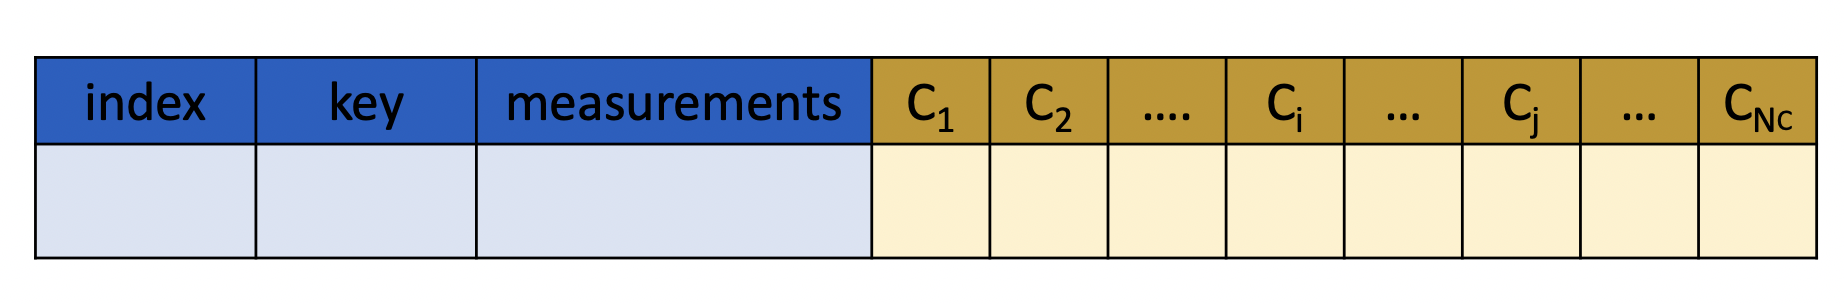
\includegraphics[width=\textwidth]{Figs/data-struc-diffcol} 

}

\caption{The data structure for exploring periodicities in data by including cyclic granularities in the tsibble structure with index, key and measured variables.}\label{fig:data-structure}
\end{figure}



\hypertarget{sec:synergy}{%
\subsection{Harmonies and clashes}\label{sec:synergy}}

The way cyclic granularities relate become important when we consider the data structure in Figure \ref{fig:data-structure}. Let us consider two cyclic granularities \(C_i\) and \(C_j\), such that \(C_i\) maps index set to a set \(\{A_k | k \in \mathbb{N}, k \leq K\}\) and \(C_j\) maps index set to a set \(\{B_l | l \in \mathbb{N}, l \leq L\}\). Here, \(A_k\)'s or \(B_l\)'s are the levels/categories corresponding to \(C_i\) and \(C_j\) respectively. Let \(S_{kl}\) be a subset of the index set such that for all \(s \in S_{kl}\), \(C_i(s) = A_k\) and \(C_j(s) = B_l\). Data subsets for each combination of levels (\(A_k\), \(B_l\)) like \textless{}\(A_k\), \(B_l\), \(v(s)\)\textgreater{} can be obtained for all \(k \in {1, 2, \dots, K}\) and \(l \in {1, 2, \dots, L}\) which will lead to \(KL\) data subsets. Now, some situations can lead to few or many of these sets being empty. We will discuss few cases, where one or more of these \(KL\) sets will be empty either due to the structure of the calendar, duration and location of events in a calendar or just by the construction of the cyclic granularities.

\begin{definition}\label{def:harmony}
A {\bf clash} is a pair of cyclic granularities which contains structurally, event-driven or build-based empty combinations of its categories.
\end{definition}

\begin{definition}\label{def:clash}
A {\bf harmony} is a pair of cyclic granularities that does not contain any empty combinations of its categories.
\end{definition}

\noindent Firstly, empty combinations can arise due to the structure of the calendar or hierarchy. These are called ``structurally'' empty combinations. Let us take a specific example, where \(C_i\) be day-of-month with 31 levels and \(C_j\) be week-of-month with 5 levels. There will be \(31\times 5=155\) sets \(S_{kl}\) corresponding to possible combinations of \(C_i\) and \(C_j\). Many of these like \(S_{1,5}\), \(S_{21,2}\) are empty. This is also intuitive since the first day of the month can never correspond to fifth week of the month. Hence the pair (day-of-month, week-of-month) is a clash.

\noindent Secondly, empty combinations can turn up due to differences in event location or duration in a calendar. These are called ``event-driven'' empty combinations. Let us consider \(C_i\) be day-of-week with 7 levels and \(C_j\) be WorkingDay/NonWorkingDay with 2 levels. While potentially all of these 14 sets \(S_{kl}\) can be non-empty (it is possible to have a public holiday on any day-of-week), in practice many of these will probably have very few observations. For example, there are few (if any) public holidays on Wednesdays or Thursdays in any given year in Melbourne, Australia.

\noindent Thirdly, empty combinations can be a result of how granularities are constructed. These are called ``build-based'' empty combinations. Let \(C_i\) be Business-days, which are days from Monday to Friday except holidays and \(C_j\) be day-of-month. Then the days denoting weekends in a month would not correspond to any Business days. This is different from structurally empty combinations because structure of the calendar does not lead to these missing combinations, but the construction of the granularities does.

\noindent An example when there will be no empty combinations could be where \(C_i\) and \(C_j\) maps index set to day-of-week and month-of-year respectively. Here \(C_i\) can have 7 levels while \(C_j\) can have 12 levels. So there are \(12\times7=84\) sets \(S_{kl}\). All of these are non-empty because every day-of-week can occur in every month. Hence, the pair (day-of-week, month-of-year) is a harmony.

\hypertarget{sec:summarize-measured}{%
\subsection{Summarizing the measured variable}\label{sec:summarize-measured}}

Restructuring time from linear to cyclic time granularities leads to re-organisation of the data structure, where each level of a cyclic granularity corresponds to multiple values of the measured variable. It is common to see summarization of these multiple values through aggregation or an unique summary statistic like mean or median to have each level of cyclic granularity correspond to an unique value of the measured variable. However, this approach hides the distributions of the measured variable induced by the re-organised data structure. Summarizing the distribution of the measured variable using these multiple observations could be a potential way to explore and bring forward different features of the data.

However, we need to consider the effect of number of observations on the summarization even for harmonies. Consider a data set with \((T + 1)\) observations, and two cyclic granularities \(C_i\) and \(C_j\) with \(K\) and \(L\) categories respectively. Let \(nobs\) be the number of observations for a combination of levels from \((C_i, C_j)\). Now, \(nobs\) might be equal for all combinations on an average so that \(nobs = (T + 1)/(KL)\) as \(T\rightarrow\infty\) or ideally take any value between \(\{0, 1, 2, \dots, T\}\). The statistical transformation used for summarizing the measured variable should be chosen in line with \(nobs\). For example, it might be useful to compute deciles for summarization only when \(nobs \ge 10\). Rarely occurring categories such as the 366th day of the year, or the 31st day of the month are likely to suffer from this problem.

\hypertarget{sec:visualization}{%
\section{Visualization}\label{sec:visualization}}

The grammar of graphics introduced a framework to construct statistical graphics by relating data space to the graphic space \citep{Wilkinson1999-nk}. The layered grammar of graphics proposed by \citet{Wickham2009pk}, which is an alternate and modified parametrization of the grammar suggests that graphics are made up of distinct layers of grammatical elements. Drawing from the grammar of graphics, if \textless{}\(C_i\), \(C_j\), \(v\)\textgreater{} serves as the basis of visualizing the distribution of the measured variable, the following layers can be specified:

\begin{itemize}
\tightlist
\item
  Data: \textless{}\(C_i\), \(C_j\), \(v\)\textgreater{}
\item
  Aesthetic mapping (mapping of variables to elements of the plot): \(C_i\) mapped to \(x\) position and \(v\) to \(y\) position
\item
  Statistical transformation (data summarization): any descriptive or smoothing statistics that summarizes distribution of \(v\)
\item
  Geometric objects (physical representation of the data): any geometry displaying distribution, for example, boxplot, letter value, violin, ridge or highest density region plots
\item
  Facet (split plots): \(C_j\)
\end{itemize}

\hypertarget{choice-of-statistical-transformations-and-geometric-objects}{%
\subsection{Choice of statistical transformations and geometric objects}\label{choice-of-statistical-transformations-and-geometric-objects}}

Choice of plots are dictated by the statistical transformations and geometric objects used for the visualization. The basic plot choice for our data structure is the one that can display distributions. We will discuss few conventional and recent ways to plot distributions using both Kernel density estimates and descriptive statistics. Descriptive statistics based displays include box plots \citep{Tukey1977-jx} or different variations of it like notched box plots \citep{Mcgill1978-hg}. More recent ways are the letter-value box plot \citep{Hofmann2017-sg} or quantile plots which display quantiles instead of quartiles in a traditional boxplot. Kernel density based plots for displaying a distribution include violin plots \citep{Hintze1998-zi}, summary plot \citep{Potter2010-qc}, ridge line plots, highest density regions (HDR) box \citep{Hyndman1996-ft}. Each type of density display has different parameters, that need to be estimated given the data. Each is equipped with some benefits and challenges which should be borne in mind while using them for exploration.

\hypertarget{facet-and-aesthetic-variables}{%
\subsection{Facet and aesthetic variables}\label{facet-and-aesthetic-variables}}

\hypertarget{sec:levels}{%
\subsubsection{Levels}\label{sec:levels}}

The levels of cyclic granularities has a role to play on the choice of plots since space and resolution might become a problem with too many levels. A potential approach could be to categorize the levels as very high/high/medium/low for each cyclic granularity and define some criteria based on usual cognitive power, display size available and the aesthetic mappings. Default values for these categorizations could be chosen based on levels of common temporal granularities like days of the month, days of the fortnight or days of the week.

\hypertarget{sec:vis-interaction}{%
\subsubsection{Synergy of cyclic granularities}\label{sec:vis-interaction}}

For data sets of the form (\(C_i\), \(C_j\), \(v\)) \(\forall i, j \in N_C\), if there are levels of \(C_i\) (or \(C_j\)) not spanned by levels of \(C_j\) (or \(C_i\)), empty sets are formed leading to potential ineffective graphs. The conjecture is that the synergy of these cyclic granularities are thus playing a role while deciding if the resulting plot would be a good candidate for exploratory analysis. Harmonies are pairs of granularities that do not contain empty combinations and could possibly be useful for exploring patterns. However, plotting clashes should be avoided since they might contain combinations which are empty or have too few observations. For illustration, \autoref{fig:allFig} (a) shows the distribution of half-hourly electricity consumption through letter value plot across months of the year faceted by quarters of the year. This plot does not work because every quarter does not correspond to all months of the year, for example, the first quarter of the year would never correspond to the month December of an year.

\begin{figure}

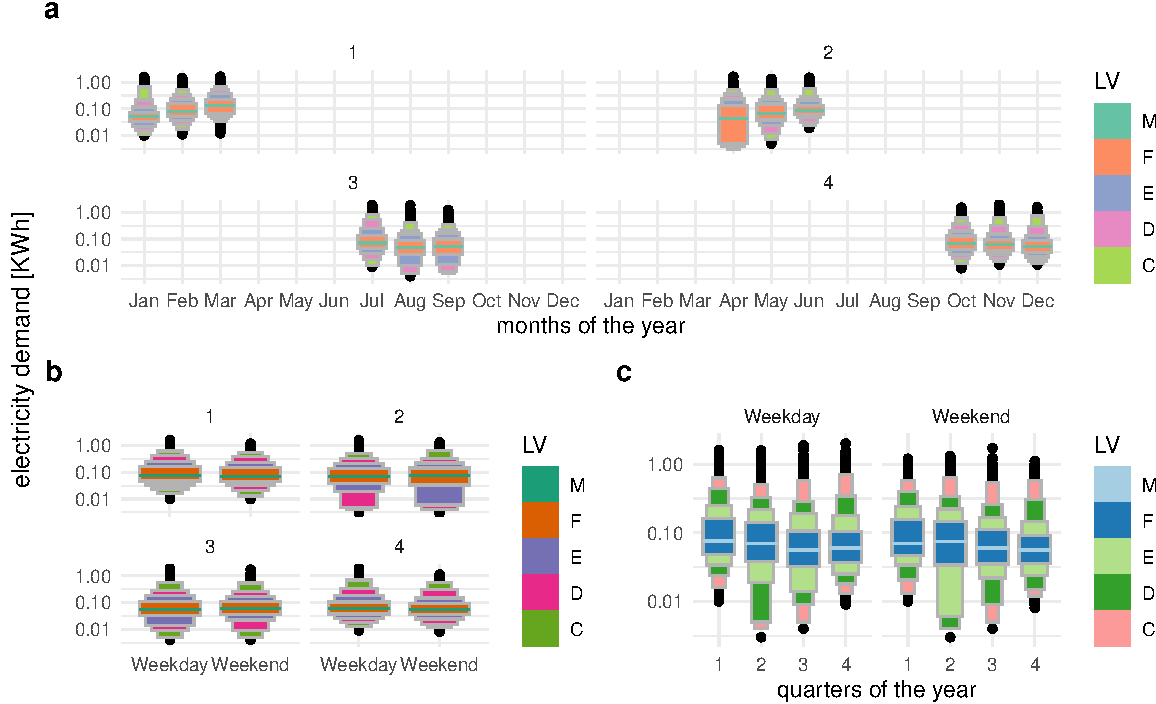
\includegraphics[width=1\linewidth]{figure/allFig-1} \hfill{}

\caption{Distribution of energy consumption displayed through letter value plots. Plot (a) displays consumption across month-of-year faceted by quarters of the year, (b) across weekday/weekend faceted by quarters of the year and (c) across quarters of the year faceted by weekday/weekend. Plots (b) and (c) both show harmonies since each quarter consists of both weekdays and weekends. Conversely, weekend and weekday can occur in every quarter. Analysts should avoid plotting such clashes. Plot (b) helps to compare weekends and weekdays for each quarter. It can be seen that for every quarter weekend and weekday consumption are fairly similar except for the second quarter where the letter values below D and E behave differently, whereas, Plot (c) helps to compare quarters within weekdays and weekends. For example, the quartile spread of consumption shrinks/lowers from first to fourth quarter for weekdays, whereas this pattern is not true for weekends. Plot (a) shows a clash since all quarters do not correspond to all months of the year.}\label{fig:allFig}
\end{figure}



\hypertarget{interchangeability-of-mappings}{%
\subsubsection{Interchangeability of mappings}\label{interchangeability-of-mappings}}

We will discuss the effect of the mapping of cyclic granularities in this section. When we consider data sets of the form \textless{}\(C_i\), \(C_j\), \(v\)\textgreater{} with \(C_i\) mapped to \(x\) position and \(C_j\) to facets, then \(A_k\)'s are placed in close proximity and each \(B_l\) represent a group/facet. Gestalt theory suggests that when items are placed in close proximity, people assume that they are in the same group because they are close to one another and apart from other groups. Hence, in this case \(A_k\)'s are compared against each other within each group. With the mapping of \(C_i\) and \(C_j\) reversed, emphasis will shift to different behavior of the variables. \autoref{fig:allFig} (b) shows the letter value plot across weekday/weekend faceted by quarters of the year and \autoref{fig:allFig} (c) shows the same two cyclic granularities with their mapping reversed. \autoref{fig:allFig} (b) helps us to compare weekday and weekend within each quarter and \autoref{fig:allFig} (c) helps to compare quarters within weekend and weekday.

\hypertarget{number-of-observations-and-statistical-transformations}{%
\subsection{Number of observations and statistical transformations}\label{number-of-observations-and-statistical-transformations}}

Visualizing distributions can be misleading if statistical transformations are performed on rarely occurring categories (Section \ref{sec:summarize-measured}). Even when there are no rarely occurring events, number of observations might vary hugely within or across each facet. This might happen due to missing observations in the data or uneven locations of events in time domain. In such cases, the statistical transformations should be used with caution as sample sizes would directly affect both the variance and consequently the confidence interval of the estimators.

\hypertarget{sec:application}{%
\section{Applications}\label{sec:application}}

\hypertarget{sec:smartmeter}{%
\subsection{Smart meter data of Australia}\label{sec:smartmeter}}

Smart meters provide large quantities of measurements on energy usage for households across Australia. One of the customer trials \citep{smart-meter} conducted as part of the Smart Grid Smart City project in Newcastle, New South Wales and some parts of Sydney provides customer wise data on energy consumption for every half hour from February 2012 to March 2014. The idea here is to show how to visualize the distribution of the energy consumption across different cyclic granularities in a systematic way to identify different behavioral patterns.

\hypertarget{cyclic-granularities-search-and-computation}{%
\subsubsection{Cyclic granularities search and computation:}\label{cyclic-granularities-search-and-computation}}

The tsibble object \texttt{smart\_meter10} from R package \texttt{gravitas} \citep{R-gravitas} consisting of \texttt{reading\_datetime}, \texttt{customer\_id} and \texttt{general\_supply\_kwh} denoting the index, key and measured variable of the tsibble is used to facilitate the systematic exploration. While trying to explore the energy behavior of these customers systematically across cyclic time granularities, the first thing to consider is which cyclic time granularities we can look at exhaustively. Let us consider conventional time deconstructions for a Gregorian calendar (second, minute, half-hour, hour, day, week, month, year). Since the interval of this tsibble is 30 minutes, the temporal granularities may range from half-hour to year. Considering \(6\) linear granularities half-hour, hour, day, week, month and year in the hierarchy table, \(N_C = (6*5/2) = 15\). If \(N_C\) seem too large, the smallest and largest linear granularities could be considered to be removed for analysis. Granularities half-year and year are removed to have \(N_C = (4*3/2) = 6\) and obtain cyclic granularities namely ``hour\_day'', ``hour\_week'', ``hour\_month'', ``day\_week'', ``day\_month'' and ``week\_month'', read as ``hour of the day'', etc. Further, we add cyclic granularity day-type( ``wknd\_wday'') to capture weekend and weekday behavior. Now that we have a list of cyclic granularities to look at, we should be able to compute them using Section \ref{sec:cyclic-calendar}.

\hypertarget{screening-and-visualizing-harmonies}{%
\subsubsection{Screening and visualizing harmonies}\label{screening-and-visualizing-harmonies}}

From the search list, \(N_C = 7\) cyclic granularities are chosen for which we would like to derive insights of energy behavior. Recalling the data structure \textless{}\(C_i\), \(C_j\), \texttt{general\_supply\_kwh}\textgreater{} for exploration \(\forall i, j \in \{1, 2, \ldots, 7\}\), each of these \(7\) cyclic granularities can either be mapped to x-axis or to facet. Choosing \(2\) of the possible \(7\) granularities, which is equivalent to having \(^{7}P_2 = 42\) candidates for visualization. Harmonies can be identified among those \(42\) possibilities to narrow the search. \autoref{tab:harmony-tab} shows \(16\) harmony pairs after removing clashes and any cyclic granularities with levels more than \(31\), as effective exploration becomes difficult with many levels (Section \ref{sec:levels}).

\noindent Few harmony pairs are displayed in \autoref{fig:bothcust} to illustrate the impact of different distribution plots and reverse mapping. For each of \autoref{fig:bothcust} (b) and (c), \(C_i\) is the circular granularity day-type (weekday/weekend) and \(C_j\) is hour of the day. The geometry used for displaying the distribution is chosen as area-quantiles and violins in \autoref{fig:bothcust} (b and c respectively). \autoref{fig:bothcust} (a) displays reverse mapping of \(C_i\) and \(C_j\) with \(C_i\) denoting hour of the day and \(C_j\) denoting day-type with distribution geometrically displayed as boxplots.
In \autoref{fig:bothcust} (b), the black line is the median, whereas the purple band covers 25th to 75th percentile, the orange band covers 10th to 90th percentile and the green band covers 1st to 99th percentile. The first facet represents the weekday behavior while the second one displays the weekend behavior and energy consumption across each hours of the day is shown inside each facet. The energy consumption is extremely (positive- or right-) skewed with the 1st, 10th and 25th percentile lying relatively close whereas 75th, 90th and 99th lying further away from each other. This is common across both weekdays and weekends. For the first few hours on weekdays, median energy consumption starts and continues to be higher for longer as compared to weekends.

\noindent Consider looking at violin plots instead of quantile plots to look at the same data in \autoref{fig:bothcust}(c) for some more insights. There is bimodality in the early hours of the day, implying both low and high energy consumption is probable in the early hours of the day both for weekdays and weekends. If we visualize the same data with reverse mapping of the cyclic granularities, then the natural tendency would be to compare weekend and weekday behavior within each hour and not across hours. For example in \autoref{fig:bothcust}(a), it can be seen that median energy consumption for the early morning hours is higher for weekdays than weekends. Also, outliers are more prominent in the latter hours of the day. All of these indicate that looking at different distribution geometry or changing the mapping might shed lights on different aspect of the energy behavior for the same sample population.

\begin{table}

\caption{\label{tab:harmony-tab}Harmonies with a pair of cyclic granularity one placed on facet and the other on x-axis. Out of 42 possible combinations of cyclic granularities, only 16 are harmony pairs.}
\centering
\begin{tabular}[t]{llrr}
\toprule
facet variable & x-axis variable & facet levels & x-axis levels\\
\midrule
day\_week & hour\_day & 7 & 24\\
day\_month & hour\_day & 31 & 24\\
week\_month & hour\_day & 5 & 24\\
wknd\_wday & hour\_day & 2 & 24\\
hour\_day & day\_week & 24 & 7\\
\addlinespace
day\_month & day\_week & 31 & 7\\
week\_month & day\_week & 5 & 7\\
hour\_day & day\_month & 24 & 31\\
day\_week & day\_month & 7 & 31\\
wknd\_wday & day\_month & 2 & 31\\
\addlinespace
hour\_day & week\_month & 24 & 5\\
day\_week & week\_month & 7 & 5\\
wknd\_wday & week\_month & 2 & 5\\
hour\_day & wknd\_wday & 24 & 2\\
day\_month & wknd\_wday & 31 & 2\\
\addlinespace
week\_month & wknd\_wday & 5 & 2\\
\bottomrule
\end{tabular}
\end{table}

\begin{figure}

{\centering 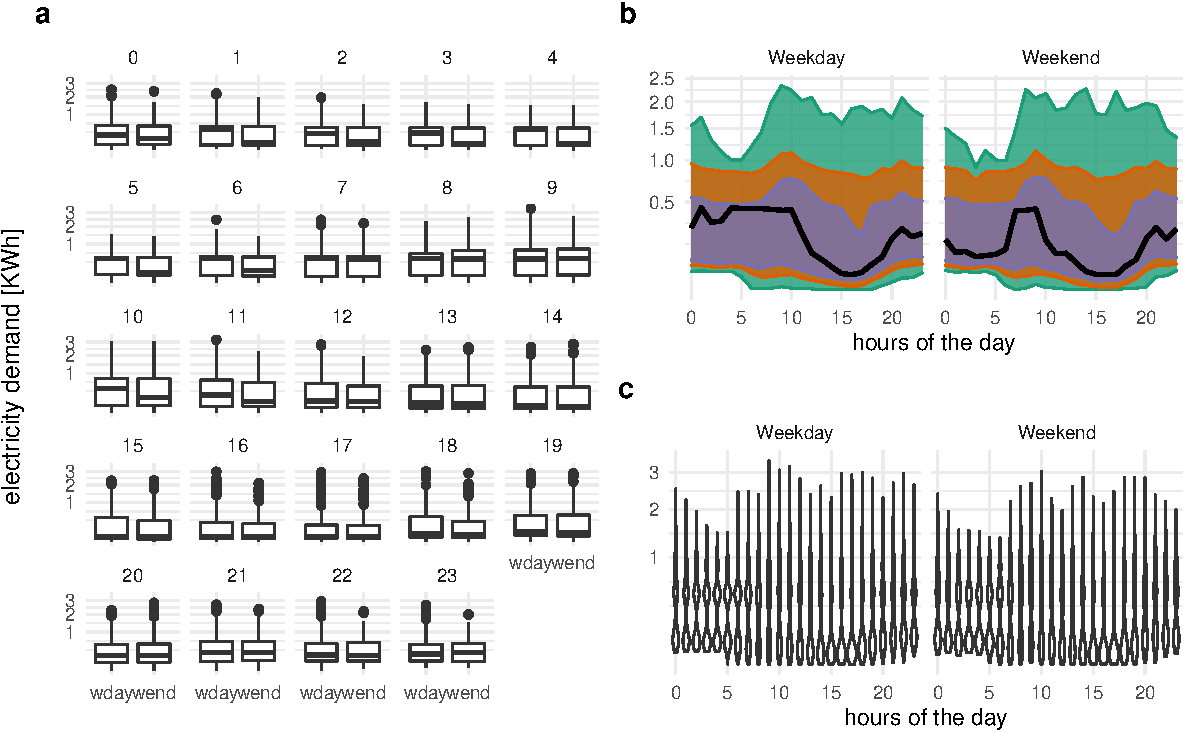
\includegraphics[width=0.9\linewidth]{figure/bothcust-1} 

}

\caption{Energy consumption of a single customer shown with different distribution displays, and granularity arrangements. Two granularities are used: hour of the day (I) and weekday/weekend (II). Plot (a) shows granularity I faceted by granularity II, and plots (b), (c) shows the converse mapping. Plot (a) makes a comparison of usage by workday within each hour of the day using side-by-side boxplots. Generally, on a work day there is more consumption early in the day. Plots (b) and (c) examine the temporal trend of consumption over the course of a day, separately for the type of day. Plot (b) uses an area quantile to put the emphasis on the time series, for example, the median consumption over time shows prolonged usage in the morning on weekdays. Plot (c) uses a violin plot to place emphasis on distributional differences across hours. It can be seen that the morning use on weekdays is bimodal, some work days there is low usage, which might indicate the person is working from home and also having a late start.}\label{fig:bothcust}
\end{figure}



If the data for all keys are visualized together, it might lead to Simpson's paradox, which occurs when one observation shows a particular behavior, but this behavior paradoxically becomes obscured by aggregation. For example in a particular neighborhood one household may have the least daily power consumption for a full week, yet still not be the household with the minimum weekly power consumption. This is an intuitive possibility, because heterogeneous \texttt{customer\_id}'s with very different occupation or demographics will tend to have very different energy behavior and combining them together will somehow weaken any typical or extreme behavior. A strategy for analyzing periodicities of multiple keys together could be to group the keys basis their energy behavior across different cyclic granularities. This is beyond the scope of the current work.

\hypertarget{sec:cricket}{%
\subsection{T20 cricket data of Indian Premiere League}\label{sec:cricket}}

The method is not only restricted to temporal data, and can be generalized to many hierarchical granularities (with continuous and uni-directional nature). We illustrate this with an application to the sport cricket. Although there is no conventional time component in cricket, each ball can be thought to represent an ordering from past to future with the game progressing forward with each ball. In the Twenty20 format, an over will consist of 6 balls (with some exceptions), an innings is restricted to a maximum of 20 overs, a match will consist of 2 innings and a season consists of several matches. Thus, similar to time, there is a hierarchy where ball is nested within overs, overs nested within innings and innings within matches. The idea of cyclic granularities can be likewise mapped to this hierarchy. Example granularites then include ball of the over, over of the innings and ball of the innings. Although most of these cyclic granularities are circular in design of the hierarchy, in application of the rules some granularities are aperiodic. For example, in most cases an over will consist of 6 balls with some exceptions like wide balls or when an innings finishes before the over finishes. Thus, the cyclic granularity ball-of-over will be circular in most cases and aperiodic in others.

\noindent The Indian Premier League (IPL) is a professional Twenty20 cricket league in India contested by eight teams representing eight different cities in India. The ball by ball data for IPL season 2008 to 2016 is fetched from \href{https://www.kaggle.com/josephgpinto/ipl-data-analysis/data}{Kaggle}. The \texttt{cricket} data set in the \texttt{gravitas} package summarizes the ball-by-ball data across overs and contains information for a sample of 214 matches spanning 9 seasons (2008 to 2016) such that each over has 6 balls, each innings has 20 overs and each match has 2 innings. This could be useful in a periodic world when we wish to compute any circular/quasi-circular granularity based on a hierarchy table which look like \autoref{tab:hierarchy-cric}. However, even if the situation is not periodic, it can be interesting to visualize the distribution of a measured variable to shed light on the aperiodic behavior of a non-temporal data set similar to aperiodic events like formal meetings, workshops, conferences, school semesters in a temporal set up.

\begin{table}

\caption{\label{tab:hierarchy-cric}Hierarchy table for cricket where overs are nested within an innings, innings nested within a match and matches within a season.}
\centering
\begin{tabular}[t]{lll}
\toprule
linear (G) & single-order-up cyclic (C) & period length/conversion operator (K)\\
\midrule
over & over-of-inning & 20\\
inning & inning-of-match & 2\\
match & match-of-season & k(match, season)\\
season & 1 & 1\\
\bottomrule
\end{tabular}
\end{table}

\noindent There are many interesting questions that could possibly be answered with the \texttt{cricket} data set. For example, it would be interesting to see if the distribution of total runs vary depending on if a team bats in the first or second innings. The Mumbai Indians (MI) and Chennai Super kings (CSK) appeared in final playoffs from 2010 to 2015. We take their example in order to dive deeper into this question. From Figure \ref{fig:cricex}(a), it can be observed that for the team batting in the first innings there is an upward trend of runs per over, while there is no clear upward trend in median and quartile deviation of runs for the teams batting in the second inning. This seem to indicate that players feel mounting pressure to score more runs as they approach towards the end of the first inning. Whereas teams batting in the second innings have a set target in mind and are not subjected to such mounting pressure and may adopt a more conservative strategy, to score runs. Thus winning teams like CSK and MI seem to employ different inning strategies when it comes to their batting order.

\noindent Another fascinating exploration would be to examine if runs per over decrease in the subsequent over if fielding (defending) was good in the previous over? For establishing the fielding quality, we apply an indicator function on dismissals (1 if there was at least one wicket in the previous over due to run out or catch, 0 otherwise). Runs in the current over is then the observation variable. Dismissals in the previous over can lead to a batsman adopting a more defensive play style. Figure \ref{fig:cricex}(b) shows that no dismissals in the previous over leads to a higher median and quartile spread of runs per over as compared to the case when there has been at least one dismissal in the previous over. Wickets per over are considered as an aperiodic cyclic granularity with wickets as an aperiodic linear granularity. These granularities do not appear in the hierarchy table since it is difficult to position them in a hierarchy. These are similar to holidays or special events in temporal data.

\begin{figure}

{\centering 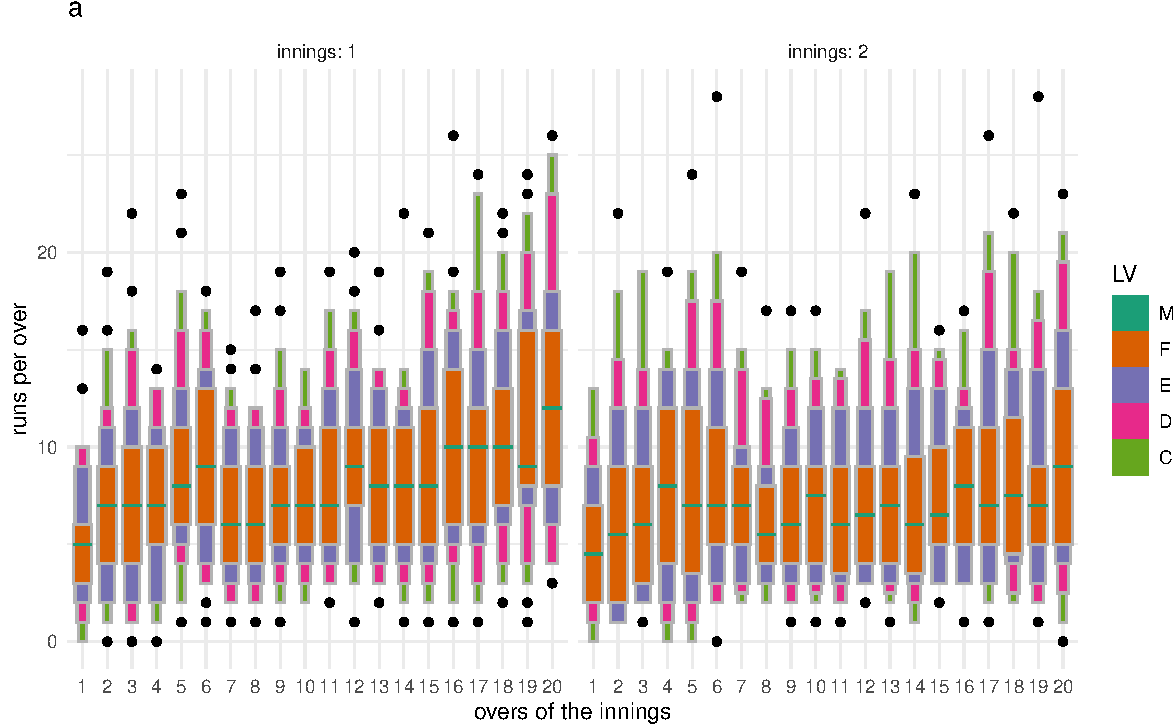
\includegraphics[width=0.9\linewidth]{figure/cricex-1} 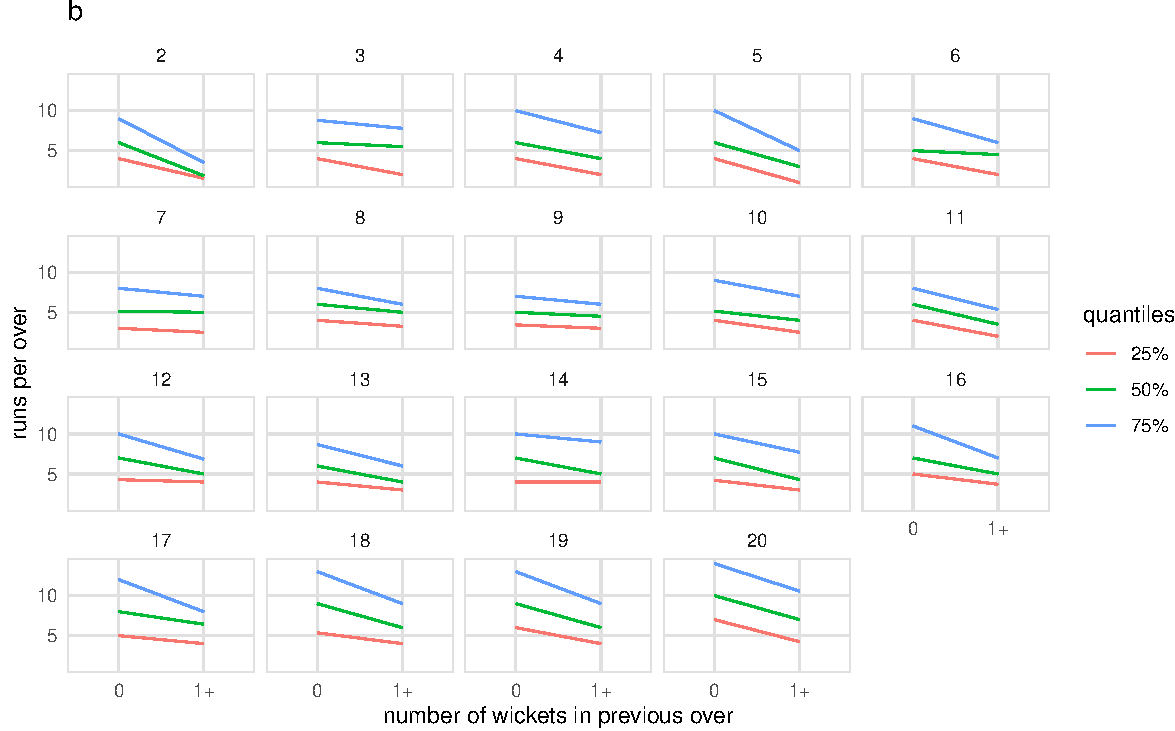
\includegraphics[width=0.9\linewidth]{figure/cricex-2} 

}

\caption{Runs per over shown with different distribution displays, and granularities. Plot (a) shows letter value plot across overs faceted by innings. For the team batting in the first innings there is an upward trend of runs per over, while there is no such pattern of runs for the teams batting in the second innings. Plot (b) shows quantile plot of runs per over across an indicator of wickets in previous over faceted by current over. This indicates that at least one wicket in the previous over leads to lower median run rate and quartile spread in the subsequent over.}\label{fig:cricex}
\end{figure}



\hypertarget{sec:discussion}{%
\section{Discussion}\label{sec:discussion}}

Exploratory data analysis and data analysis in general involve many iterations of finding and summarizing patterns. With temporal data available at ever finer scales, exploring periodicity can become overwhelming with so many possible granularities to explore. This work provides a framework to systematically explore distribution of an univariate measured variable across two cyclic time granularities by creating any cyclic granularity, ranking a list of harmonies and thereby identifying possible distribution plots for effective visualization based on relationship and levels of the cyclic granularities.

A missing piece in the package \texttt{gravitas} is the computation of cyclic aperiodic granularities which would require computing aperiodic linear granularities first. A few R packages like \texttt{almanac} and \texttt{gs} provide functionality to create recurring events that are not periodic. These functions can be imported in the \texttt{gravitas} package to accommodate for aperiodic cyclic granularities. Another future direction of work could be to further refine the search of harmonies by only selecting pairs of cyclic granularities for which variation in measured variable is significant and rating these selected harmony pairs in order of importance for exploration.

\hypertarget{acknowledgements}{%
\section*{Acknowledgements}\label{acknowledgements}}
\addcontentsline{toc}{section}{Acknowledgements}

The authors would like to thank the cohort \href{https://www.monash.edu/news/articles/team-profile-monash-business-analytics-team}{NUMBATS}, Monash University for sharing their wisdom and experience of developing R packages and Dr.~Peter Toscas \href{https://data61.csiro.au/}{from Data61 CSIRO} for providing useful inputs on improving the analysis of smart meter application. The package \texttt{gravitas} was built during the \href{https://summerofcode.withgoogle.com/archive/}{Google Summer of Code, 2019}. We would also like to thank Nicholas Spyrison for many useful discussions, sketching figures and feedback on the manuscript. More details about the package can be found on the package website \href{https://sayani07.github.io/gravitas/}{sayani07.github.io/gravitas}. This article was created with \texttt{knitr} \citep[\citet{R-knitr}]{knitr2015} and \texttt{rmarkdown} \citep[\citet{R-rmarkdown}]{rmarkdown2018}. This paper's Github repository, \href{https://github.com/Sayani07/paper-gravitas}{github.com/Sayani07/paper-gravitas}, contains all materials required to reproduce this article and the code is also available online in the supplemental materials.

\hypertarget{supplemental-materials}{%
\section{Supplemental Materials}\label{supplemental-materials}}

\textbf{Data and scripts:} Data sets and R code to reproduce all figures in this article (main.Rmd).

\textbf{R-package:} The ideas presented in this article have been implemented in the open-source R \citep{R-language} package \texttt{gravitas} \citep{R-gravitas}, available from CRAN. The R-package facilitates manipulation of single and multiple-order-up time granularities through cyclic calendar algebra, check feasibility of creating plots or drawing inferences for any two cyclic granularities by providing list of harmonies and recommend prospective probability distributions through factors described in the article. Version 0.1.2 of the package was used for the results presented in the article and is available on Github (\url{https://github.com/Sayani07/gravitas}).

\textbf{R-packages:} Each of the R packages used in this article are available online with URLs provided in the bibliography.

\bibliographystyle{agsm}
\bibliography{bibliography.bib}

\end{document}
